\textbf{Ejemplo 4:}\\
Una entidad estatal puede usar el edificio A que requiere 5.000.000 COP cada año como costo de mantenimiento y  6.000.000 COP cada 5 años para reparaciones, o puede usar el edificio B, que requiere  5.100.000 COP cada año como costo de funcionamiento y  1.000.000 COP cada 2 años para reparaciones. Suponiendo una tasa de $j=30\%$ nominal anual año vencido y que el edifico escogido se ocupara por tiempo indefinido, ¿cuál de los dos edificios le resulta más conveniente utilizar?\\

\textbf{Solución:}

%La tabla ira centrada
\begin{center}
 \renewcommand{\arraystretch}{1.5}% Margenes de las celdas
 %Creación de la cuadricula de 3 columnas
 \begin{longtable}[H]{|c|c|c|}
  %Creamos una linea horizontal
  \hline
  %Definimos el color de la primera fila
  \rowcolor[HTML]{FFB183}
  %%%%% INICIO ASIGNACIÓN FECHA FOCAL %%%%%%%
  %%%%%%%%%% INICIO TITULO
  %Lo que se hace aquí es mezclar las 3 columnas en una sola
  \multicolumn{3}{|c|}{\cellcolor[HTML]{FFB183}\textbf{1. Asignación período focal}}\\ \hline
  \multicolumn{3}{|c|} {$pf=0\textit{ pav}$}\\ \hline
  %%%%%%%%%% FIN TITULO
  %%%%% INICIO DECLARACIÓN DE VARIABLES %%%%%%%
  %%%%%%%%%% INICIO TITULO
  %Lo que se hace aquí es mezclar las 3 columnas en una sola
  \multicolumn{3}{|c|}{\cellcolor[HTML]{FFB183}\textbf{2. Declaración de variables}}\\ \hline
  %%%%%%%%%% FIN TITULO
  %%%%%%%%%% INICIO DE MATEMÁTICAS
  %Cada & hace referencia al paso de la siguiente columna
  \multicolumn{2}{|l|}{$R_{a_1}=5{.}000{.}000\,\,COP\textit{ matenimiento cada año}$} & $VP_a= ?\,\,COP$   \\
  \multicolumn{2}{|l|}{$R_{a_2}=6{.}000{.}000\,\,COP\textit{ reparacion cada 5 años}$} & $VP_b= ?\,\,COP$   \\
  \multicolumn{2}{|l|}{$R_{b_1}=5{.}100{.}000\,\,COP\textit{ matenimiento cada año}$} & \\
  \multicolumn{2}{|l|}{$R_{b_2}=1{.}000{.}000\,\,COP\textit{ reparación cada 2 años}$} & \\ \hline
  
  %%%%% INICIO FLUJO DE CAJA
  \rowcolor[HTML]{FFB183}
  \multicolumn{3}{|c|}{\cellcolor[HTML]{FFB183}\textbf{3. Diagrama de flujo de caja}}
  \\ \hline
  %Mezclamos 3 columnas y pondremos el dibujo
  %%%%%%%%%%%%% INSERCIÓN DE LA IMAGEN
  %Deberán descargar las imágenes respectivas del drive y pegarlas en la carpeta
  %n_capitulo/img/ejemplos/1/capitulo1ejemplo1.pdf  (el /1/ es el numero del ejemplo)
  \multicolumn{3}{|c|}{ 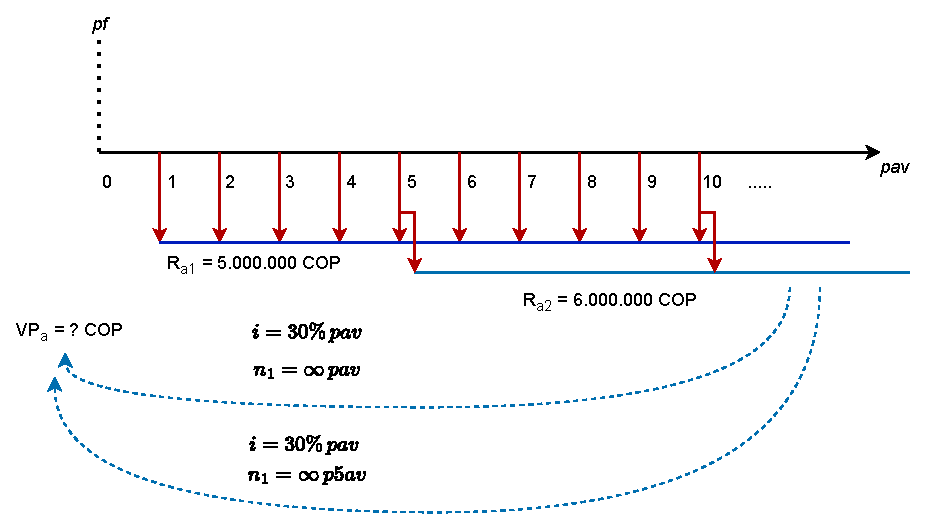
\includegraphics[trim=-5 -5 -5 -5 , max width=250px, max height=350px]{5_Capitulo/ejemplos/4/Capitulo5Ejemplo4-1.pdf} }\\
  \multicolumn{3}{|c|}{ 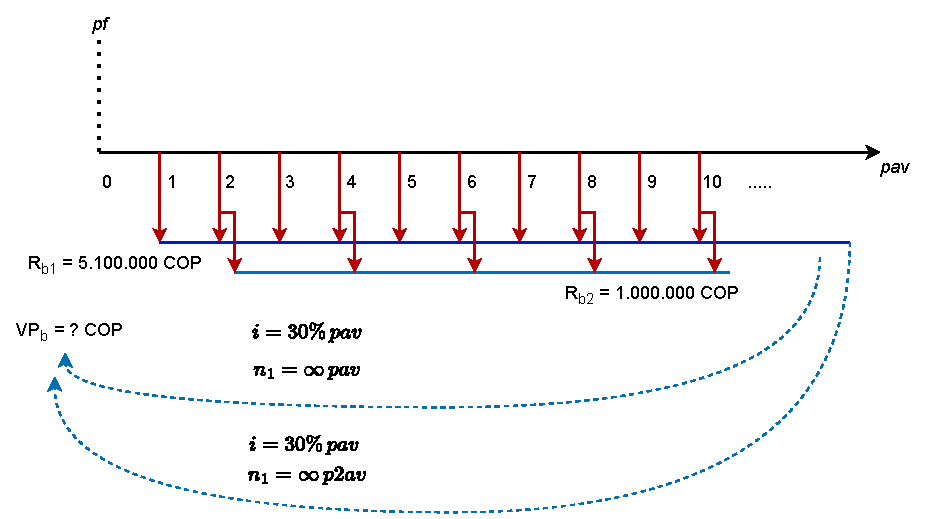
\includegraphics[trim=-5 -5 -5 -5 , max width=250px, max height=350px]{5_Capitulo/ejemplos/4/Capitulo5Ejemplo4-2.pdf} }\\
  \hline
  %%%%%%%%%%%%% FIN INSERCIÓN DE IMAGEN
  %%%%%FIN FLUJO DE CAJA  
  
  %%%%% INICIO DECLARACIÓN FORMULAS
  %%%%%%%%%%% INICIO TITULO
  \rowcolor[HTML]{FFB183}
  \multicolumn{3}{|c|}{\cellcolor[HTML]{FFB183}\textbf{4. Declaración de fórmulas}}\\ \hline
  %%%%%%%%%%% FIN TITULO
  %%%%%%%%%%% INICIO MATEMÁTICAS
  
  \multicolumn{3}{|c|}{$VF=R(\frac{(1+i)^n-1}{i}) \hspace{0.4 cm} \textit{Valor futuro de una serie uniforme vencida}$}\\
  \multicolumn{3}{|c|}{$VP=\frac{R}{i} \hspace{0.4 cm} \textit{Valor presente de una serie uniforme vencida perpetua}$}\\
  \hline
  
  %%%%%%%%%% FIN MATEMÁTICAS
  %%%%%% INICIO DESARROLLO MATEMÁTICO
  \rowcolor[HTML]{FFB183}
  %%%%%%%%%%INICIO TITULO
  \multicolumn{3}{|c|}{\cellcolor[HTML]{FFB183}\textbf{5. Desarrollo matemático}}\\ \hline
  %%%%%%%%%% FIN TITULO
  %%%%%%%%%% INICIO MATEMÁTICAS
  \multicolumn{3}{|l|}{\textbf{Para el edificio A:}}\\
  \multicolumn{3}{|p{\textwidth}|}{Cálculo del valor presente de la serie uniforme vencida perpetua del costo anual de mantenimiento:}\\
  \multicolumn{3}{|c|}{$VP_{a_1}=\frac{5{.}000{.}000\,\,COP}{0.3\,pav}\hspace{0.2 cm}\rightarrow \hspace{0.2 cm}VP_{a_1}=16{.}666{.}666.67\,\,COP$}\\
  \multicolumn{3}{|p{\textwidth}|}{Cálculo de la R anual equivalente de la serie quinquenal de reparación.}\\
  \multicolumn{3}{|c|}{$6{.}000{.}000\,\,COP=R_{R_{a2}}(\frac{(1+0.3)^5-1}{0.3})\hspace{0.2 cm}\rightarrow \hspace{0.2 cm}R_{R_{a2}}=663{.}489\,\,COP$} \\
  \multicolumn{3}{|p{\textwidth}|}{Cálculo del valor presente de la serie uniforme vencida anual perpetua equivalente por la reparación.}\\
  \multicolumn{3}{|c|}{$VP_{a_2}=\frac{663{.}490\,\,COP}{0.3}\hspace{0.2 cm}\rightarrow \hspace{0.2 cm}VP_{a_2}=2{.}211{.}631\,\,COP$}\\
  \multicolumn{3}{|c|}{$VP_{a}=16{.}666{.}667\,\,COP+2{.}211{.}631\,\,COP\hspace{0.2 cm}\rightarrow \hspace{0.2 cm}VP_{a}=18{.}878{.}798\,\,COP$}\\
  \multicolumn{3}{|l|}{\textbf{Para el edificio B:}}\\
  \multicolumn{3}{|p{\textwidth}|}{Se repiten los mismos cálculos:}\\
  \multicolumn{3}{|c|}{$VP_{a_1}=\frac{5{.}100{.}000\,\,COP}{0.3}\hspace{0.2 cm}\rightarrow \hspace{0.2 cm}VP_{b_1}=17{.}000{.}000\,\,COP$}\\
  \multicolumn{3}{|c|}{$1{.}000{.}000\,\,COP=R_{R_{b2}}(\frac{(1+0.3)^2-1}{0.3})\hspace{0.2 cm}\rightarrow \hspace{0.2 cm}R_{R_{b2}}=434{.}783\,\,COP$} \\
  \multicolumn{3}{|c|}{$VP_{b_2}=\frac{434{.}783\,\,COP}{0.3}\hspace{0.2 cm}\rightarrow \hspace{0.2 cm}VP_{b_2}=1{.}449{.}275\,\,COP$}\\
  \multicolumn{3}{|c|}{$VP_{b}=17{.}000{.}000\,\,COP+1{.}449{.}275\,\,COP\hspace{0.2 cm}\rightarrow \hspace{0.2 cm}VP_{b}=18{.}449{.}275\,\,COP$}\\
  \multicolumn{3}{|c|}{$VP_a-VP_b=18{.}878{.}798\,\,COP-18{.}449{.}275\,\,COP=429{.}522\,\,COP\hspace{0.2 cm}$}\\
  \hline

  %%%%%%%%%% FIN MATEMÁTICAS
  %%%%%% FIN DESARROLLO MATEMÁTICO
  %%%%%% INICIO RESPUESTA
  \rowcolor[HTML]{FFB183}
  %%%%%%%%%%INICIO TITULO
  \multicolumn{3}{|c|}{\cellcolor[HTML]{FFB183}\textbf{6. Respuesta}}\\
  \hline
  %%%%%%%%%% FIN TITULO
  %%%%%%%%%% INICIO RESPUESTA MATEMÁTICA
  \multicolumn{3}{|p{\textwidth}|}{\centering{Es conveniente hacer uso del edificio B, que representa un ahorro de $429{.}522\,\,COP$}}
  \\ \hline
  %%%%%%%%%% FIN MATEMÁTICAS
  %%%%%% FIN RESPUESTA
 \end{longtable}
 %Se crean dos lineas en blanco para que no quede el siguiente texto tan pegado
 %\newline \newline %USARLO SI CREES QUE ES NECESARIO
\end{center}
%%%%%%%%%%%%%%%%%%%%%%%%%%FIN EJERCICIO 4 %%%%%%%%%%%%%%%%%%%%%%%%%%%
